
\documentclass[12pt]{article}
\usepackage[utf8]{inputenc}


\usepackage[margin=1.1 in]{geometry}
\usepackage[T1]{fontenc}
\usepackage{mathtools}   % loads »amsmath«
\usepackage{amssymb}
\usepackage{amsfonts}
\usepackage{amsmath}
\usepackage{amsthm}
\usepackage{xcolor}
\usepackage{cancel}
%\usepackage{graphics}
\usepackage{graphicx}
%others
\usepackage{enumerate}
\usepackage{subcaption}
\usepackage{booktabs}



\usepackage{apacite}
\usepackage[round]{natbib}
%\bibliographystyle{plainnat}
\bibliographystyle{apacite}

\DeclarePairedDelimiter{\ceil}{\lceil}{\rceil}

\setlength{\parskip}{0.005em}
\usepackage{setspace}
%\singlespacing
\spacing{1.15}



\newtheorem{defin}{Definition.}
\newtheorem{teo}{Theorem. }
\newtheorem{lema}{Lemma. }
\newtheorem{coro}{Corolary. }
\newtheorem{prop}{Proposition. }
\theoremstyle{definition}
\newtheorem{examp}{Example. }
\newtheorem{problem}{}

\title{An SMM estimation of search cost in banking services: A Monte Carlo study}
\author{Giselle Labrador Badia}
\date{May 2022}

\begin{document}

\maketitle

\section{Introduction}
\section{Simulated Method of Moments}
The estimator chosen in the most important part of this exercise is simulated method of moments estimator:
$$ \text{argmin}_\theta \quad (\hat{g} - \hat{g}(\theta))'W(\hat{g} - \hat{g}(\theta))$$
where $\hat{g}$ are the moments from the original data, $\hat{g}(\theta)$ are the simulated moments, and the weight matrix $W$ is any positive semidefinite matrix. I made the exercises shown below using the matrix that contains the inverse of the data moments in the diagonal and zeroes otherwise. 

\section{Model}

This is a model of search for banking services like mortgages, credit cards, and other loans. What is special about these markets is that consumers need to search for prices and prices vary not only because of search frictions but because consumers' willingness to pay is different and depends on income, risk, and creditworthiness.

Consumers start with a home bank $h \in J$ from which they easily can get offers and quotes.  Consumers then should decide whether to search ($d=1$) for information about another bank's offers, which is costly. If the individual does not search it settles with the home bank $h$ and $d=0$.  In this model there will be two banks, that is, $J = \{ \1,2}$. Consumers are randomly assigned with probability $p$ to bank 1 as the initial bank, otherwise, their financial institution is bank 2.  Consumer $i$ utility from dealing with home bank $h \in J$ is
$$u_{hi} = v_h - p_{ih}$$
where $v_h$ is the valuation for bank $i$ which is known and bank-specific, and $p_\{ih\}$ is the quote  from bank $h$ to consumer $i$.

Consumer $i$ utility from searching and choosing bank $j \in J$ (that might be homebank as well) is
$$u^d_{ji}} = v_j - p_{ij} - k$$
where $v_j$ is the valuation for bank $i$ which is known and bank-specific, and $p_\{ih\}$ is the quote obtained from bank $h$ to consumer $i$.

Consumers characteristics are they creditworthiness $x$, and the price of a consumer $i$ in bank $j$ is 
$$p_{ij} = \alpha_j + \beta_j x_i + \varepsilon_{ij}$
where $\alpha_j$ the constant maximum loan banks can give, $\beta_{j}\leq 0 $ is how much banks penalize a low creditworthiness. The idiosyncratic error $\varepsilon_{ij}$ distributes multivariate normal with $\mu =(0,0)$ and covariance matrix $\Sigma$. See that a low creditworthiness will be linked to a higher price that is worst for consumers.

Consumers have a prior about $\alpha_j$ and $\beta_j$. This unknown coefficients are drawn from uniform distributions and are independent from each other. Individual rational choice for the simple case that $\rho = 0$ (we do not condition on $p_{hi}$) is to search ($d= 1$)  when
$$u_{ih} < \mathbb{E}[u^d_{ij}]$$
and not to search ($d= 0$) otherwise.
See that $\mathbb{E}[u^d_{ij}] = v_j - \mathbb{E}{\alpha_j} -\mathbb{E}{\beta_j} x_i$ 
 After an individual search, she chooses the bank that gives her the higher utility and pays the search cost $k$. The bank that the consumer chooses whether there was a search or not is denoted by $b$, and it is $b = 1$ if it was bank 1 and $b = 0$ if it was bank 2. See from the inequality before that consumers don't know the actual value of $\alpha_j$ and $\beta_j$ or their individual $\epsilon_{ij}$ when choosing whether to search or not. Hence, many times they will search and will remain with their home bank. 


We do not know in general what would have been optimal for consumers, to search or not to search. We do not know either what utility is higher $u_{ih}$ or $u^d_{ij}$.  The econometrician only observes if the consumer changes bank (choose the service from the other bank $j \neq h$), I call this variable $c$. Therefore if a change was observed I know that the price offered by the chosen bank was better. However, we do not see if it was optimal for consumers to search ex-post because the cost of search might be higher than the differences in prices even when there was a change in banks. 

We don't observe what are the two quotas offered by both banks. We only observe the quotes from the final bank $b$.
$$b = z * (1 - c) + (1 - z) * c $$
Let $p$ denote the observed price vector for all consumers, that is 
$$p = p_1 * b + p_2 * (1-b)$$


\section{Identification}

In principle, I could estimate $\Sigma$ but for this exercise, I focus on the estimation of the bank coefficients $\alpha_j$ and $\beta_j$ and especially on the estimation of the search parameter $k$. For this exercise, another important simplifying assumption is that agents are homogeneous in search cost. Another possibility would have been to have discrete types of consumers or $k \sim F(k)$.

As final quotes, we are seeing quotes that are consistently lower since the agent choose the final quote. More likely this is due to agents' disinformation about $\alpha$ and $\beta$, so we will see more of the best bank to make deals with. A small part of it is from the idiosyncratic error $\varepsilon$ which makes it more likely individuals got a high draw of $\varepsilon$ that they choose this bank. More importantly, since this error does not depend on creditworthiness $x$, OLS conditions are met and we have an unbiased consistent estimator.

We can discuss two settings, one in which search is observed and one in which it is not. For the estimation of $\alpha_j$ and $\beta_j$, this is not crucial. However, for the estimation of the search parameter $k$ by simulated method of moments, this considerably diminishes the number of moments available. For the estimations below I assume that the search is observable and consider the full set of moments. I use up to 24 moments (table below) to identify and estimate the parameters.  This estimator is consistent because the number of moments is always greater than the number of parameters.



Another assumption I make is making the variance of the dispersion in prices from two banks the same. Zero correlation will make banks' decisions about consumers uncorrelated beside $x$. Positive correlation makes sense if these banks care about the same unobservables and negative correlation otherwise. More notably, because the parameter of interest is $k$, I assume this is known by the econometrician.

\section{Estimation}

Parameters and primitives initial values:

\begin{itemize} 
    \itemsep0em 
    \item $\lambda = 0.01$
    \item $x \sim \text{Exponential}(\lambda)$
    \item $v_1$ = 20 
    \item $v_2$ = 18
    \item $p = 0.5$
    \item $\alpha_1 \sim U[15,25]$
    \item $\alpha_2 \sim U[19,23]$
    \item $\beta_1 \sim U[-0.1,0]$
    \item $\beta_2 \sim U[-0.1,0]$
    \item $\sigma_1 = \sigma_2 = 0.5$
    \item $\rho = 0$
    \item $k = 1.0$
\end{itemize}



\subsection{Estimation of $\alpha_j$ and $\beta_j$}

Since, these parameters are drawn from uniform distributions so in principle in each simulation will have different values, I decided to use fix parameters unobservables for consumers to estimate this part.
\begin{itemize}
    \itemsep0em 
    \item $\alpha_1 = 21$ (for simulations)
    \item $\alpha_2 = 23$ (for simulations)
    \item $\beta_1 = -0.03$  (for simulations)
    \item $\beta_2 = -0.07$  (for simulations)
\end{itemize}
In the first step, I estimate via OLS the parameters of the price equation for each firm. Notice that econometricians only observe prices from the final bank $b$. Below I show the result of the regressions. The estimates from the OLS regressions are significant and pretty close to the estimands.  

\begin{table}[h]
\centering
\begin{tabular}{rrrrr}
\toprule
 & True Bank 1 & True Bank 2 & Bank 1 estimates & Bank 2 estimates\\
\midrule
 \alpha & 21.0 & 23.0 & 21.09 & 22.73\\
&  &  & (0.0001832) & (0.0005507)\\
 \beta & -0.03 & -0.07 & -0.03318 & -0.06902\\
 &  & & (4.741e-8) & (1.112e-8)\\
\bottomrule
\end{tabular}
\caption{Regression results two OLS regressions of the two firms. }
\end{table}

\subsection{Estimation of search cost $k$}

The true value of $k$ is 1. 
\begin{table}
\centering
\begin{tabular}{rrrr}
\toprule
 & Moments & Mean & Description\\
\midrule
1 & E[d] & 0.557 & Percent of individuals who search.\\
2 & E[c] & 0.389 & Percent of individuals who change banks.\\
3 & E[d|b=1] & 0.41 & Expectation of search conditional on bank 1 being chosen.\\
4 & E[d|b=0] & 0.817 & Expectation of search conditional on bank 2 being chosen.\\
5 & E[c|b=1] & 0.404 & Expectation of change conditional on bank 1 being chosen.\\
6 & E[c|b=0] & 0.363 & Expectation of change conditional on bank 2 being chosen.\\
7 & E[d|z=1] & 0.264 & Expectation of search conditional on homebank being bank 1.\\
8 & E[d|z=0] & 0.865 & Expectation of search conditional on homebank being bank 2.\\
9 & E[c|z=1] & 0.256 & Expectation of change conditional on homebank being bank 1.\\
10 & E[c|z=0] & 0.529 & Expectation of change conditional on homebank being bank 2.\\
11 & E[p] & 15.806 & Expectation of price\\
12 & E[b] & 0.639 & Percent of individuals that choose bank 1\\
13 & E[p|d=0] & 16.669 & Expectation of price conditional on no search\\
14 & E[p|d=1] & 15.119 & Expectation of price conditional on search\\
15 & E[p|c=0] & 16.188 & Expectation of price conditional on no change\\
16 & E[p|c=1] & 15.205 & Expectation of price conditional on change\\
17 & V[p|d=0] & 45.287 & Variance of price conditional on no search\\
18 & V[p|d=1] & 46.028 & Variance of price conditional on search\\
19 & V[p|c=0] & 35.702 & Variance of price conditional on no change\\
20 & V[p|c=1] & 62.352 & Variance of price conditional on change\\
21 & E[p1] & 19.424 & Expectation of price bank 1\\
22 & E[p2] & 9.4 & Expectation of price bank 2\\
23 & V[p1] & 2.174 & Variance of price bank 1\\
24 & V[p2] & 60.094 & Variance of price bank 2\\
\bottomrule
\end{tabular}
\caption{Moments used on estimation.}
\end{table}

The number of replications for each simulation design was 30. The number of moments considered was 1, 2, 3, 4, and 24, and the number of individuals considered in each simulation was 500, 1000, 2000, and 5000. This took a long time because of the computational complexity of the task. With more time it will be interesting to try another intermediary number of moments like 10, 15, or 20. In table 3 we see how as $n$ increases and $m$ increases, the estimation improves significantly. The estimation with the lower $n$ is very poor no matter how many moments and standard errors are larger. With large $n$ even when we use only one moment (just-identified) we get pretty good estimates. Interestingly we do not see any difference in mean estimates when we go from $m=1$(just-identified) to $m =2$(over-identified), we do get a closer best fit since there are more combinations of moments. However, I don't think this is critical since when using real data we won't know what the moments that will give us estimates closer to the real parameters are.  

\begin{table}[]
    \centering
\begin{tabular}{r|ccccc}
\toprule
               & m=1      & m=2         & m=3         & m=4         & m=24        \\ \hline
     $\hat{k}$ &    0.859 &       0.859 &       0.857 &       0.867 &       0.882 \\
               &  (0.007) &     (0.007) &     (0.002) & (7.849e-04) & (3.302e-04) \\
$max(\hat{k})$ &    1.019 &       1.005 &       0.994 &       0.994 &       0.991 \\
             n &  500.000 &     500.000 &     500.000 &     500.000 &     500.000 \\ \hline
     $\hat{k}$ &    0.986 &       0.986 &       0.987 &       0.989 &       1.005 \\
               &  (0.002) & (4.662e-04) & (1.539e-04) & (5.542e-05) & (1.237e-16) \\
$max(\hat{k})$ &    1.005 &       1.001 &       1.001 &       1.001 &       1.005 \\
             n & 1000.000 &    1000.000 &    1000.000 &    1000.000 &    1000.000 \\ \hline
     $\hat{k}$ &    1.006 &       0.993 &       0.995 &       0.996 &       0.998 \\
               &  (0.003) & (3.542e-04) & (1.110e-04) & (3.829e-05) & (1.031e-16) \\
$max(\hat{k})$ &    1.001 &       1.001 &       1.001 &       1.001 &       0.998 \\
             n & 2000.000 &    2000.000 &    2000.000 &    2000.000 &    2000.000 \\ \hline
         $\hat{k}$ &    0.968 &       1.003 &       1.003 &       1.003 &       1.005 \\
               &  (0.006) & (9.710e-05) & (2.985e-05) & (1.002e-05) & (1.237e-16) \\
$max(\hat{k})$ &    1.001 &       1.001 &       1.001 &       1.001 &       1.005 \\
             n & 5000.000 &    5000.000 &    5000.000 &    5000.000 &    5000.000 \\
\bottomrule
\end{tabular}
\caption{Simulated mean, standard error and best fit from different simulation designs for true value of $k=1$.}
\end{table}

 
\begin{figure}[h]
\centering
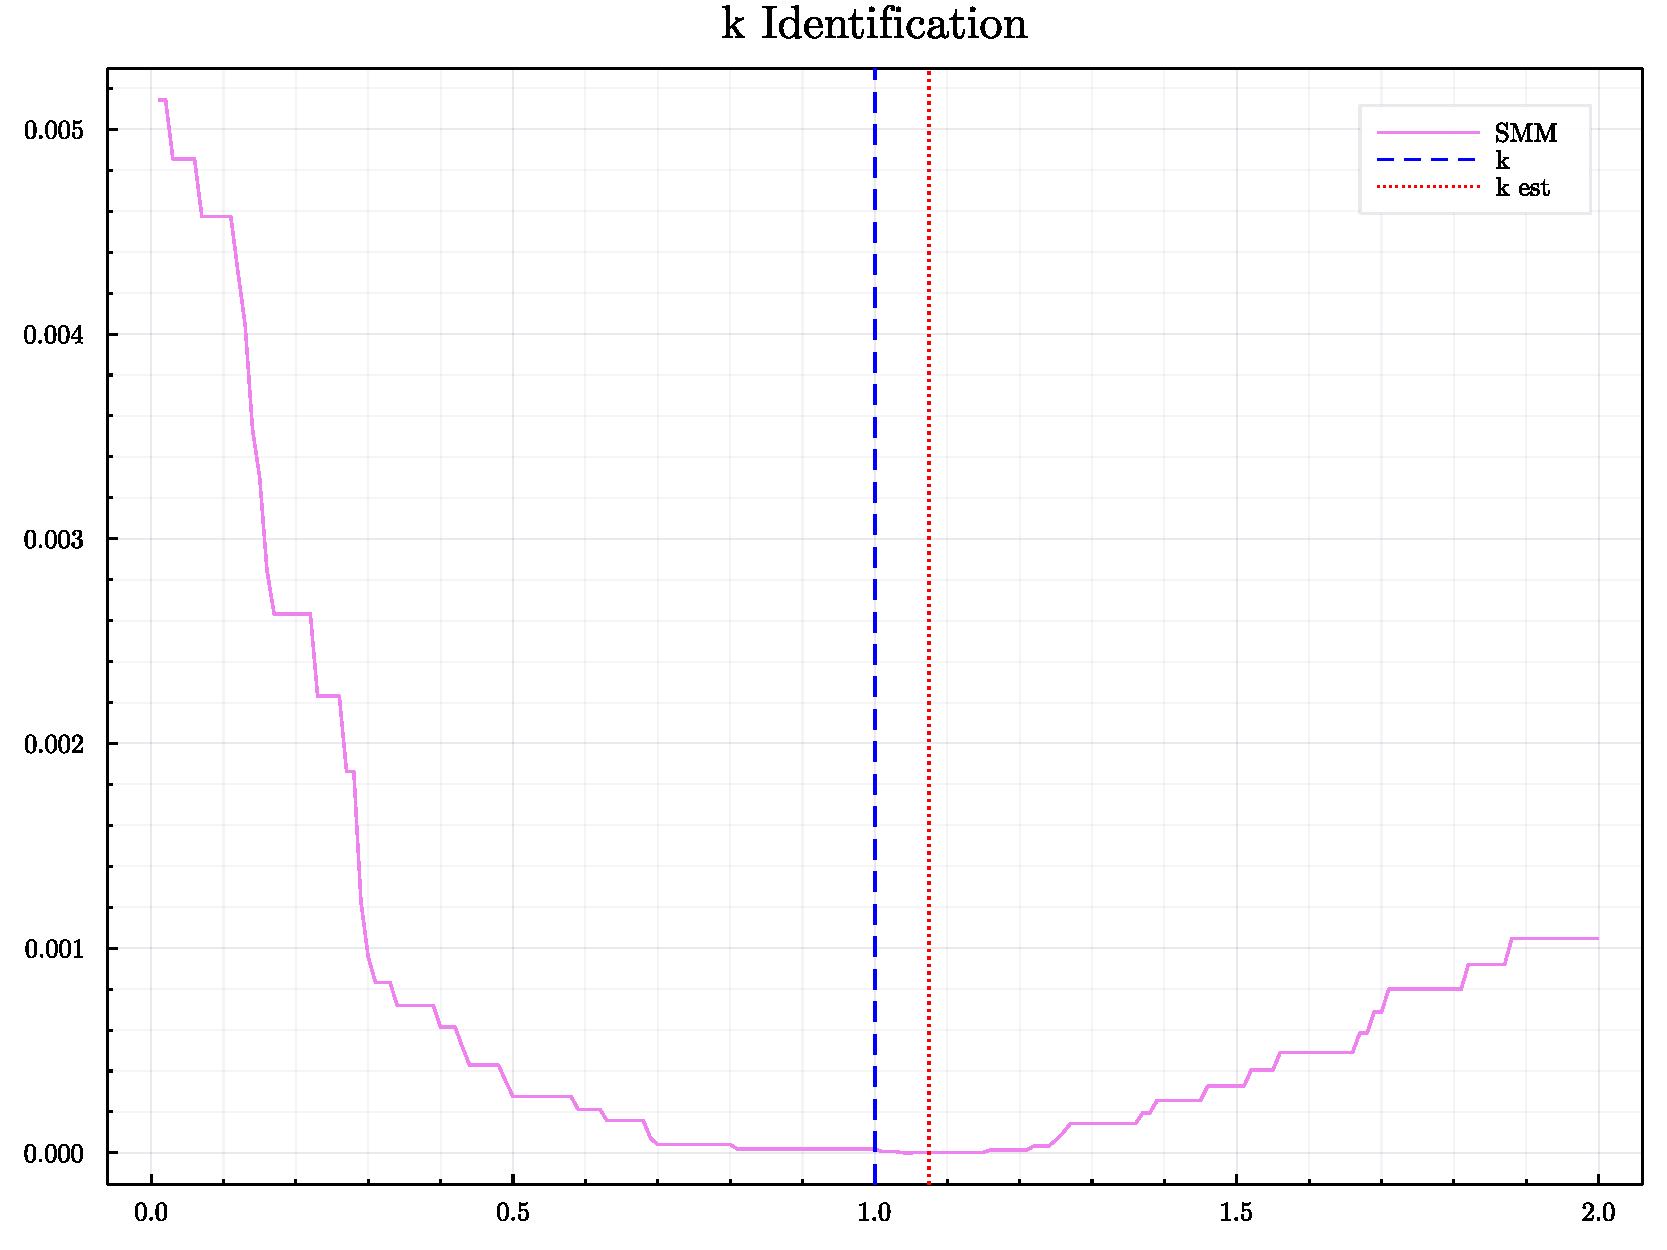
\includegraphics[width=11cm]{MonteCarlo_final/imgs/kfit_n500_m1_d_z=1.pdf}
\caption{Fit using one moment ($E[d|z=1]$) and $n = 500.$}
\end{figure}

\begin{figure}[h]
\centering
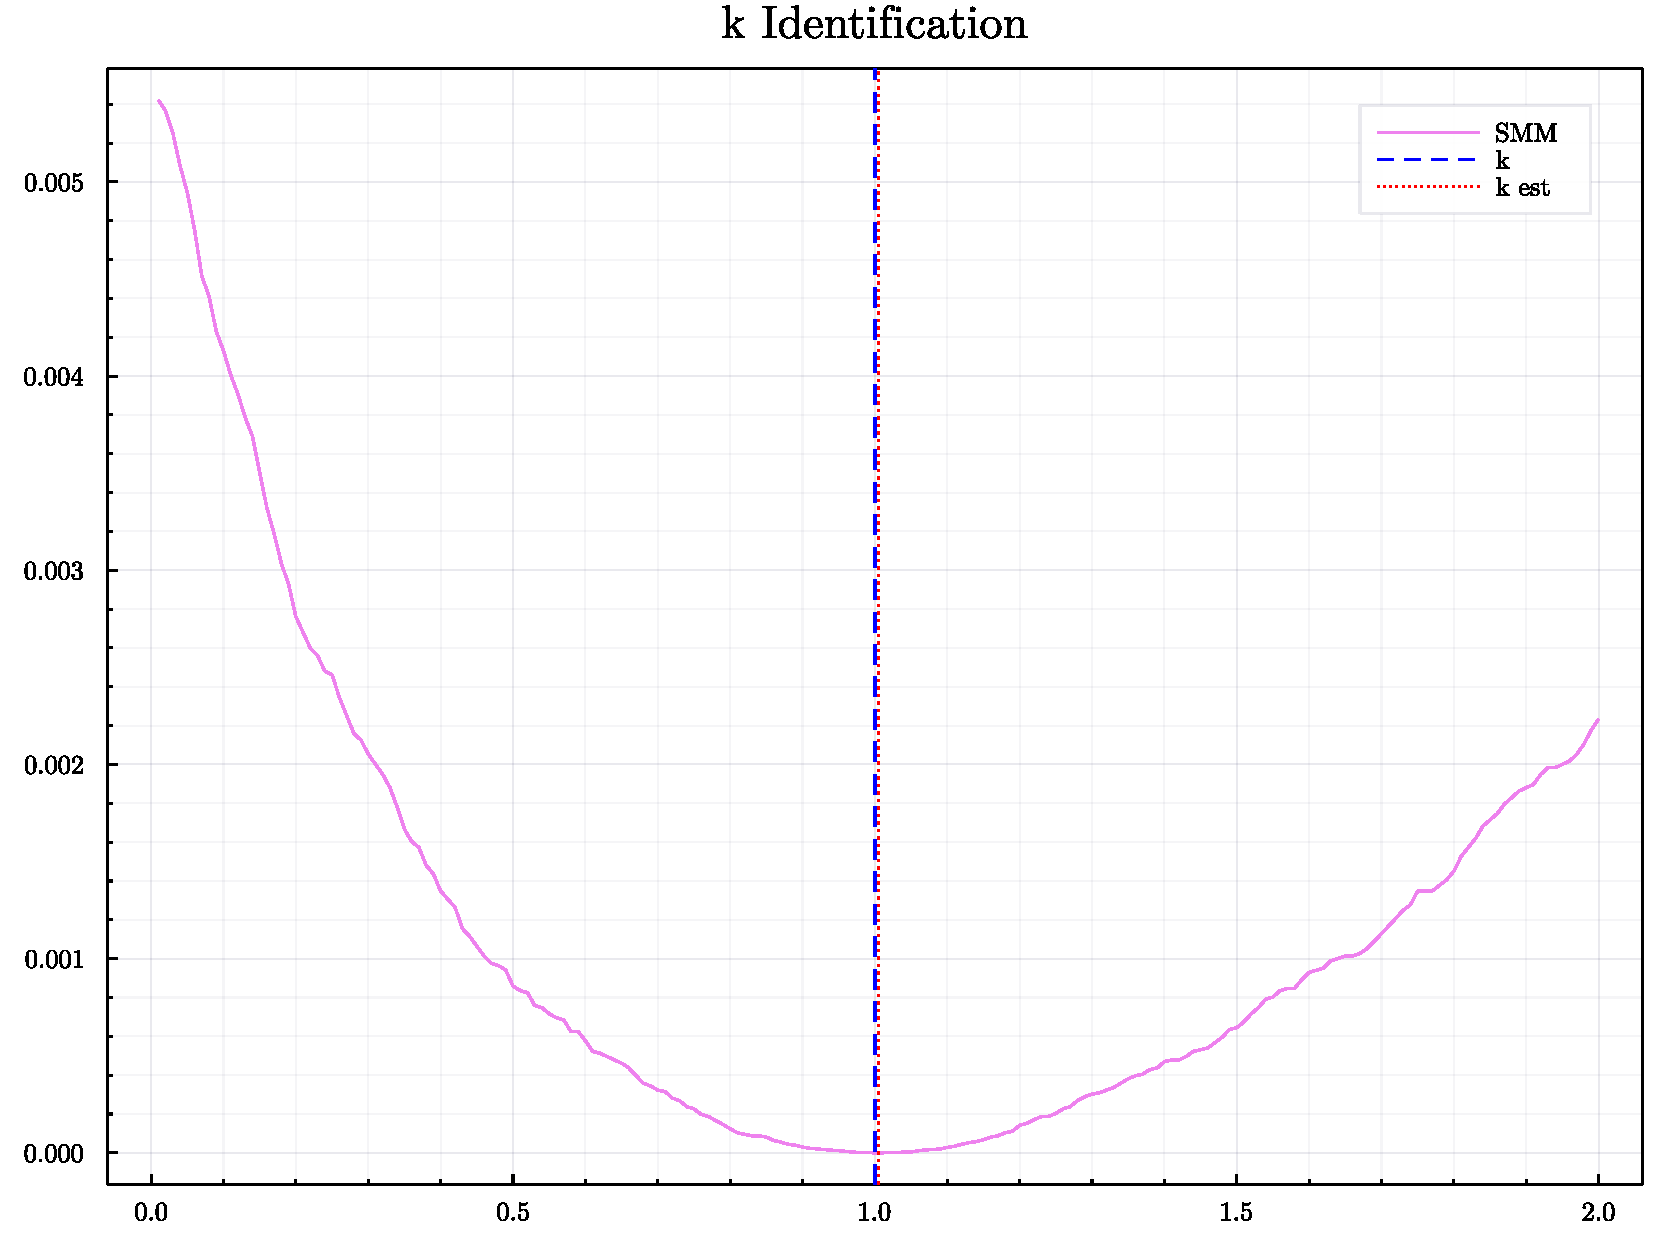
\includegraphics[width=11cm]{MonteCarlo_final/imgs/kfit_n5000_m1_d_z=1.pdf}
\caption{Fit using one moment ($E[d|z=1]$) and $n = 5000.$}
\end{figure}

\begin{figure}[h]
\centering
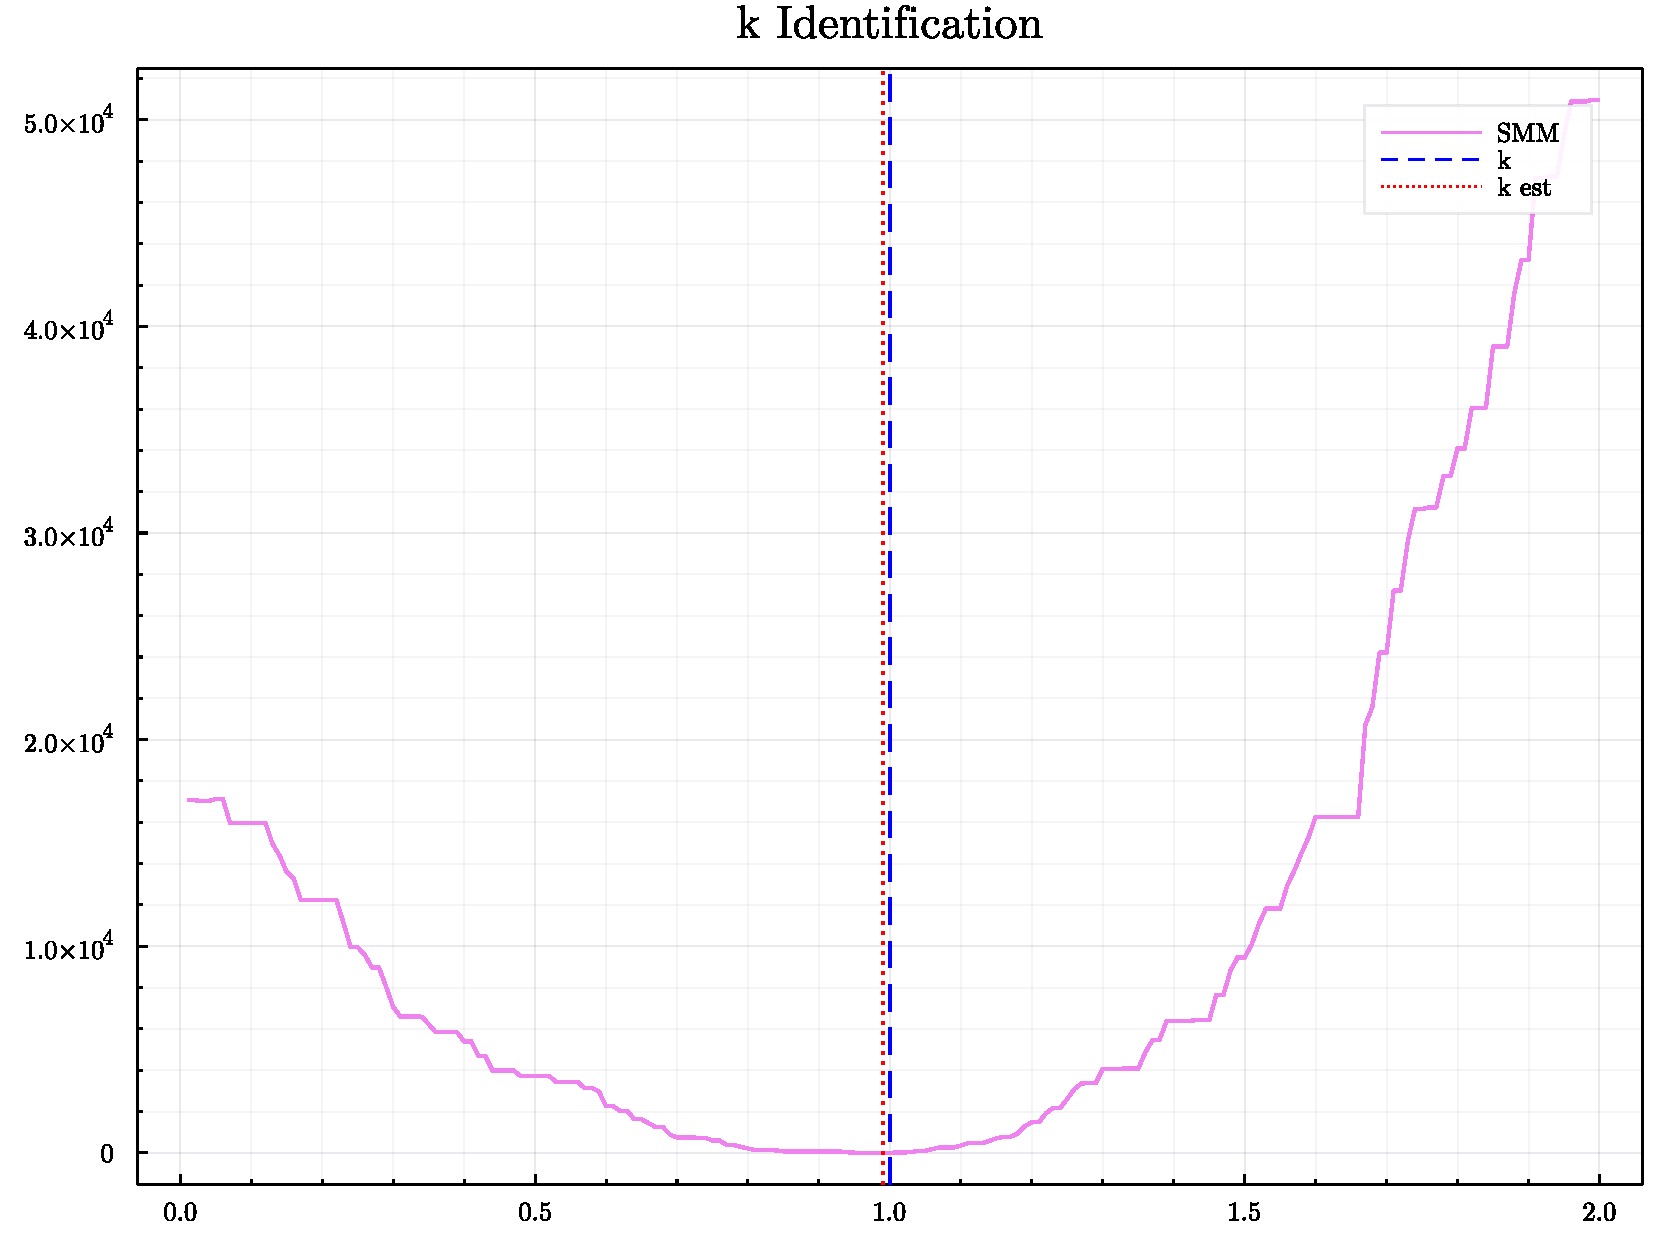
\includegraphics[width=11cm]{MonteCarlo_final/imgs/kfit_n500_m24.pdf}
\caption{Fit using all 24 moments and $n = 500.$}
\end{figure}

\begin{figure}[h]
\centering
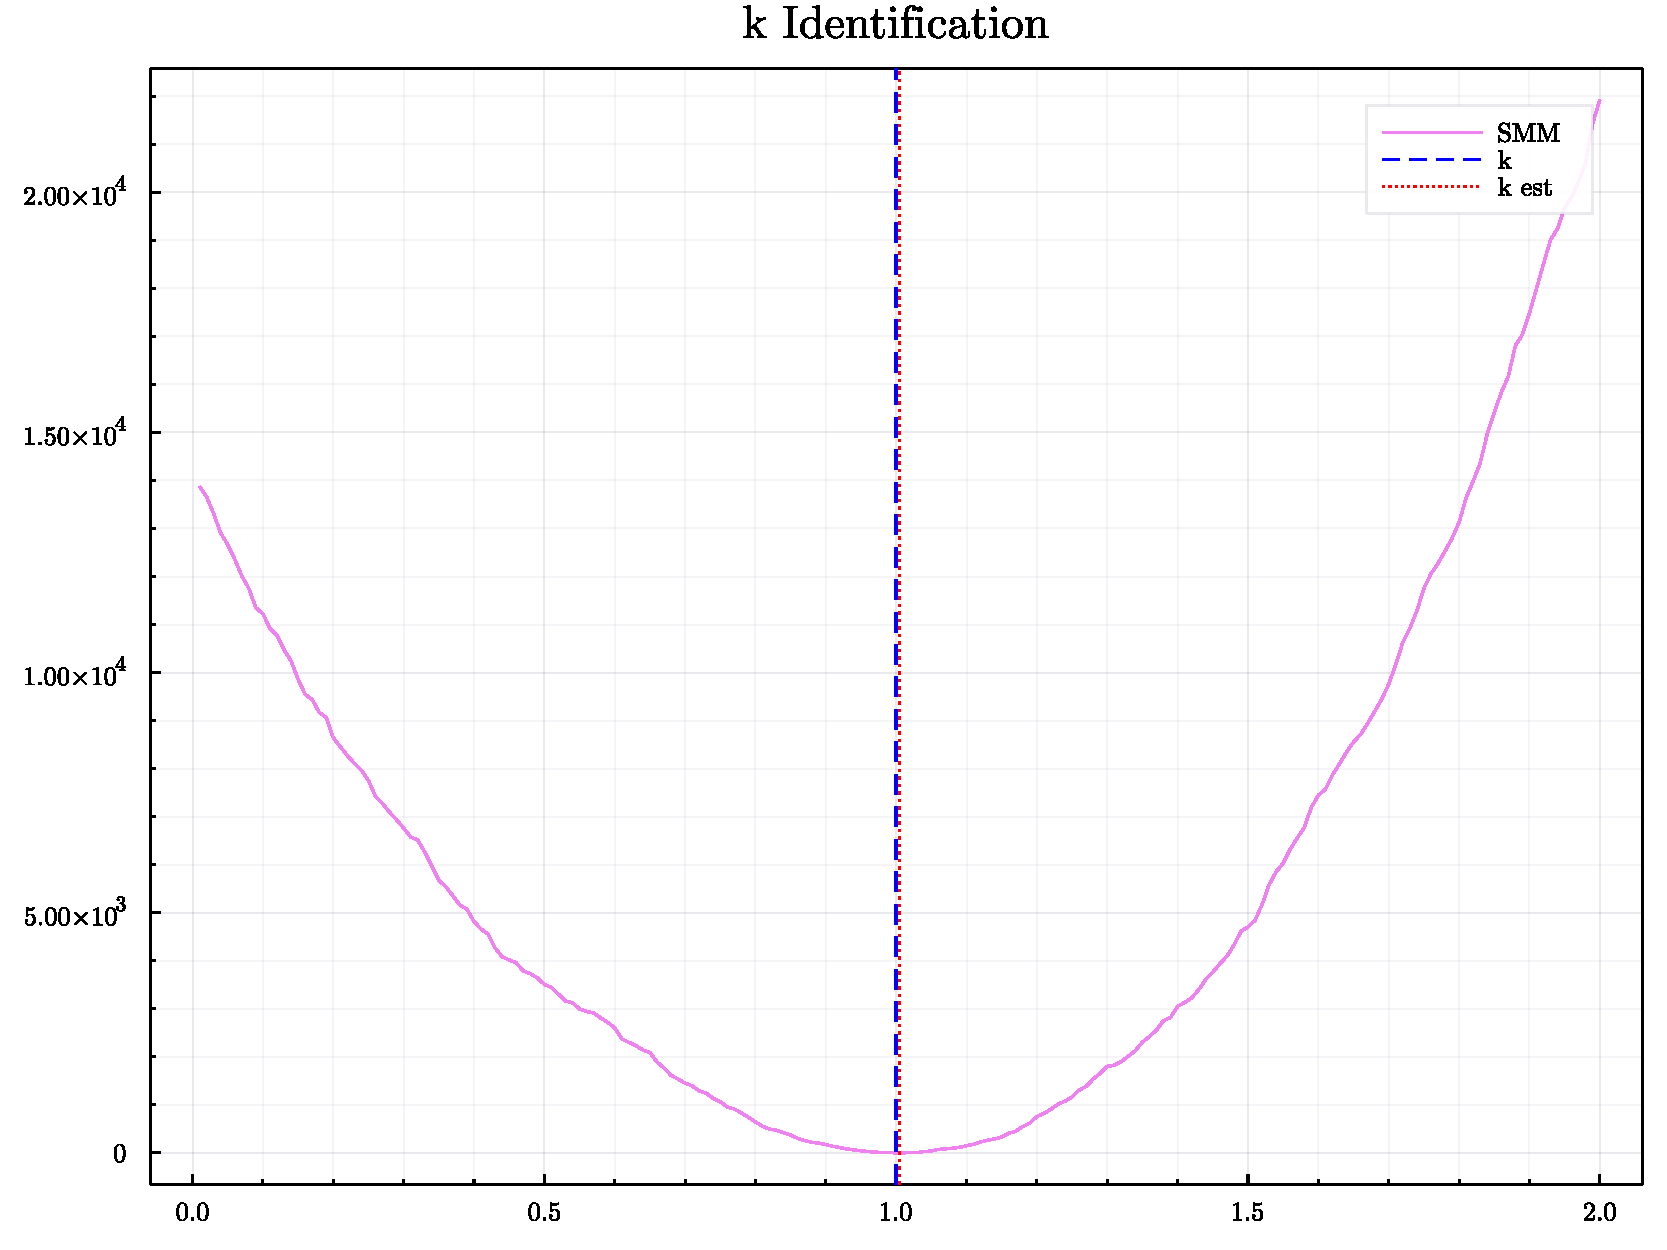
\includegraphics[width=11cm]{MonteCarlo_final/imgs/kfit_n5000_m24.pdf}
\caption{Fit using all 24 moments and $n = 5000.$}
\end{figure}


\section{Discussion}

\end{document}